\chapter{Wiederholung}
\renewcommand{\chaptertitle}{Wiederholung}


\lehead[]{\sf\hspace*{-2.00cm}\textcolor{white}{\colorbox{lightblue}{\parbox[c][0.70cm][b]{1.60cm}{
\makebox[1.60cm][r]{\thechapter}\\ \makebox[1.60cm][r]{ÜBUNG}}}}\hspace{0.17cm}\textcolor{lightblue}{\chaptertitle}}
\rohead[]{\textcolor{lightblue}{\chaptertitle}\sf\hspace*{0.17cm}\textcolor{white}{\colorbox{lightblue}{\parbox[c][0.70cm][b]{1.60cm}{\thechapter\\
ÜBUNG}}}\hspace{-2.00cm}}
%\chead[]{}
\rehead[]{\textcolor{lightblue}{AvHG, Inf, My}}
\lohead[]{\textcolor{lightblue}{AvHG, Inf, My}}

\section{Java}

\subsection{Aufgabe 1: String-Manipulationen}

\begin{center}
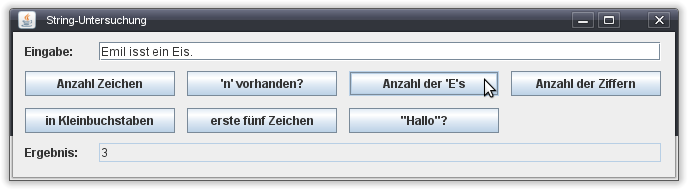
\includegraphics[width=0.9\textwidth]{./inf/SEKII/39_Java_UML_Wiederholung/StringManipulationen.png}
\end{center}

\begin{compactenum}[a)]
\item Baue die abgebildete Oberfläche nach. Das untere Textfeld soll nicht
editierbar sein. Dieses Textfeld dient zur Ausgabe der Ergebnisse.

\item Wenn der Benutzer auf den Button \glqq Anzahl Zeichen\grqq\ klickt, wird
die Anzahl der Zeichen im Eingabetextfeld ermittelt. Das Ergebnis wird im
unteren Textfeld ausgegeben.

\item Wenn der Benutzer auf den Button \glqq 'n' vorhanden?\grqq\ klickt, wird
untersucht, ob in der Zeichenkette im oberen Textfeld ein 'n' vorkommt. Das
Ergebnis (\glqq ja\grqq\ oder \glqq nein\grqq ) wird im unteren Textfeld
ausgegeben.

\item Wenn der Benutzer auf den Button \glqq Anzahl 'E's\grqq\ klickt, wird
gezählt, wie viele kleine oder große 'E's in der Zeichenkette im Eingabetextfeld
vorkommen. Das Ergebnis wird im unteren Textfeld ausgegeben.

\item Wenn der Benutzer auf den Button \glqq Anzahl der Ziffern?\grqq\ klickt,
wird gezählt, wie viele Ziffern (Zahlen zwischen 0 und 9) in der Zeichenkette
im Eingabetextfeld vorkommen. Das Ergebnis wird im unteren Textfeld ausgegeben.

\item Wenn der Benutzer auf den Button \glqq in Kleinbuchstaben\grqq\ klickt,
werden alle Buchstaben des Eingabetextes in Kleinbuchstaben umgewandelt. Das
Ergebnis wird im unteren Textfeld ausgegeben.

\item Wenn der Benutzer auf den Button \glqq erste 5 Zeichen\grqq\ klickt,
werden die ersten fünf Zeichen aus dem String im Eingabetextfeld heraus geholt
und in das untere Textfeld geschrieben. Falls dabei ein Fehler auftritt wird in
das untere Textfeld geschrieben: \glqq Der Text ist zu kurz.\grqq .

\item Wenn der Benutzer auf den Button \glqq Hallo?\grqq\ klickt, wird
untersucht, ob im Eingabetextfeld der String \glqq Hallo\grqq\ steht. Das
Ergebnis (\glqq ja\grqq\ oder \glqq nein\grqq ) wird im unteren Textfeld
ausgegeben.
\end{compactenum}


\subsection{Aufgabe 2: Count Down (Thread-Übung)}

Erstelle ein Anwendungsfenster mit einem einzigen, nicht editierbaren Textfeld,
in dem zu Beginn die Zahl 10 steht. In einem Thread wird die Zahl im
Sekundentakt um eins herunter gezählt. Wenn der Wert 0 erreicht ist, wird das
Anwendungsfenster rot eingefärbt (mit der JFrame-Methode
\lstinline|setBackground()|) und der Thread beendet sich.

\begin{center}
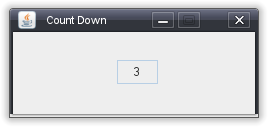
\includegraphics[width=0.45\textwidth]{./inf/SEKII/39_Java_UML_Wiederholung/CountDown.png}
\end{center}


\subsection{Brötchenbestellung}

Erstelle die abgebildete Programmoberfläche:

\begin{center}
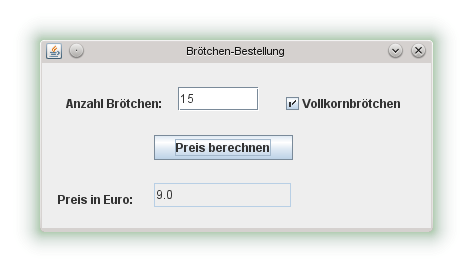
\includegraphics[width=0.55\textwidth]{./inf/SEKII/39_Java_UML_Wiederholung/Broetchenbestellung.png}
\end{center}

Wenn man auf den Button \glqq Preis berechnen\grqq\ drückt, wird der Preis für
die gewünschte Anzahl Brötchen bestimmt. Dazu wird zuerst überprüft, ob der
Benutzer eine korrekte Zahl eingegeben hat (einen Integer-Wert, der größer als
Null ist). Falls nicht wird in einer Messagebox eine geeignete Fehlermeldung
ausgegeben. Falls die Eingabe korrekt ist, wird abgefragt, ob das Häkchen bei
\glqq Vollkornbrötchen\grqq\ gesetzt ist. Für Vollkornbrötchen beträgt der Preis
0,60 € pro Stück. Für normale Brötchen zahlt man nur 0,30 € pro Stück.

Tipp: Nutze aus, dass die Methode \lstinline|Integer.parseInt()| eine
\myClass{NumberFormatException} erzeugt, wenn der eingegebene String nicht in
eine ganze Zahl umgewandelt werden kann.


\subsection{Aufgabe 4: Lauftext (Thread-Übung)}

Erstelle ein Anwendungsfenster mit einem nicht editierbaren Textfeld, das zu
Beginn leer ist. Im Sekundentakt sollen die Buchstaben des Wortes
\glqq Abrakadabra\grqq\ einfliegen (\glqq A\grqq , \glqq Ab\grqq , \glqq
Abr\grqq , \glqq Abra\grqq , und so weiter).

Schreibe das Wort \glqq Abrakadabra\grqq\ dazu in eine String-Variable und
programmiere den Code so, dass er auch funktioniert, wenn ein anderes Wort in
der Variable steht.


\subsection{Aufgabe 5: Steinen ausweichen}

Im Kursrepository findest du die Klasse \myClass{Mann} mit folgendem Code:

\begin{lstlisting}
import java.awt.*;

public class Mann {
    int x;
    int y;

    public Mann(int x, int y) {
        this.x = x;
        this.y = y;
    }

    public void zeichnen(Graphics g) {
æ        // Kopf
æ        g.setColor(Color.ORANGE);
        g.fillOval(x + 10, y, 20, 20);
æ        // Bauch
æ        g.setColor(Color.BLUE);
        g.fillOval(x + 10, y + 20, 20, 30);
æ        // Arme
æ        g.drawLine(x, y + 40, x + 20, y + 20);
        g.drawLine(x + 20, y + 20, x + 40, y + 40);
æ        // Beine
æ        g.drawLine(x + 20, y + 40, x + 10, y + 70);
        g.drawLine(x + 20, y + 40, x + 30, y + 70);
    }
}
\end{lstlisting}

\begin{center}
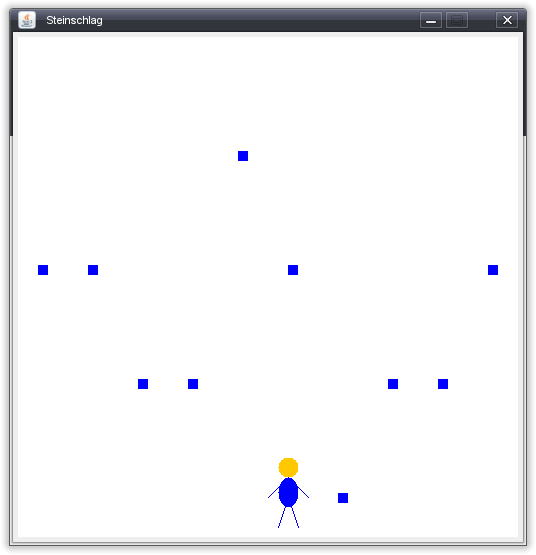
\includegraphics[width=0.65\textwidth]{./inf/SEKII/39_Java_UML_Wiederholung/FallendeSteine.png}
\end{center}

\begin{compactenum}[a)]
\item Erzeuge ein neues Anwendungsfenster mit einer Zeichenfläche, die eine
Breite und Höhe von je 500 Pixeln hat. Erzeuge und zeichne im Anwendungsfenster
ein Objekt der Klasse \myClass{Mann} an der Position (250, 420).

\item Programmiere einen Timer-Thread, der die \lstinline|repaint()|-Methode des
Anwendungsfensters alle 20 Millisekunden aufruft. Der Thread soll gleich zu
Beginn des Programms gestartet werden und die ganze Zeit durchlaufen.

\item Der Mann soll sich nun auf Tastendruck bewegen.

Wenn der Benutzer den Buchstaben 'r' (für rechts) drückt, beginnt der Mann eine
Bewegung nach rechts. Seine x-Position soll dabei wiederholt um zwei Pixel nach
rechts verschoben werden, bis der Benutzer einen anderen Buchstaben drückt.
Wenn der Benutzer den Buchstaben 'l' (für links) drückt, bewegt sich der Mann
wiederholt um zwei Pixel nach links. Wenn der Benutzer ein 's' (für stopp)
drückt, steht der Mann still.

\item Der Mann besitzt eine Breite von 40 Pixeln. Der Benutzer muss den Mann so
steuern, dass er immer im Fenster bleibt. Wenn sich einer der Arme des Mannes
außerhalb des Fensters befindet, soll die Anwendung beendet werden. Dazu musst
du den Code

\begin{lstlisting}
System.exit(0);
\end{lstlisting}

aufrufen.

\item Vom Himmel sollen Steine fallen, denen der Mann ausweichen muss.

Programmiere dazu eine neue Klasse \myClass{Stein}.

Dem Stein werden im Konstruktor seine x-Position, seine Geschwindigkeit und ein
Verweis auf den Mann als Parameter übergeben. Die y-Position des Steins wird zu
Beginn fest auf den Wert 0 gesetzt.

Zeichne den Stein als ausgefülltes schwarzes Quadrat mit einer Breite und Höhe
von zehn Pixeln. Lass den Stein außerdem bei jedem Aufruf der Methode
\lstinline|zeichnen()| entsprechend seiner Geschwindigkeit ein Stück nach unten
fallen.

Wenn der Stein aus dem Fenster heraus gefallen ist, wird er automatisch wieder
nach oben positioniert, so dass er erneut herunterfallen kann.

Erzeuge im Anwendungsfenster ein Array von zehn Steinen. Der erste Stein soll
die x-Position 20 haben. Die anderen Steine sollen jeweils im Abstand von 50
Pixeln folgen. Übergib den Steinen für die Geschwindigkeit Zufallswerte
zwischen eins und vier.

\item Wenn einer der Steine den Mann trifft, ist das Spiel vorbei und die
Anwendung soll mit \lstinline|System.exit(0);| beendet werden. Dazu vergleicht
jeder Stein in der \lstinline|zeichnen()|-Methode seine eigene Position mit der
Position des Mannes. Der Stein trifft den Mann, wenn die y-Position seiner
unteren Kante größer als 420 ist, und wenn sich entweder seine linke oder seine
rechte Seite innerhalb der 40 Pixel großen Ausdehnung des Mannes befindet.
\end{compactenum}


\section{UML-Zustandsdiagramme}

\subsection{Aufgabe 1: Hausbau}

Als Teil eines größeren Computerspiels wird eine Gruppe von Handwerkern
modelliert, die ein Haus aufbauen. Beschreibe die Zustände eines einzelnen
Handwerkers in einem UML-Zustandsdiagramm:

\begin{quotation}
\noindent
Ein Handwerker hackt zuerst im Wald einen Stapel Holz, dann läuft er mit dem
Holz zur Baustelle und baut die Balken ein. Wenn das Haus noch nicht fertig
ist, läuft er anschließend wieder zurück zum Wald um neues Holz zu hacken und
beginnt den Arbeitszyklus von vorne.

\noindent
Falls das Haus fertig ist, bleibt der Handwerker untätig neben dem Haus stehen.
Wird das Haus von Feinden zerstört, so läuft er wieder zum Wald und beginnen
erneut mit Holzhacken, um das Haus wieder aufzubauen.
\end{quotation}


\subsection{Aufgabe 2: Igelspiel}

\textbf{Ziel des Spieles}: 

Der Igel steht am linken Rand des Fensters und muss bis zum rechten Rand des
Fensters laufen ohne von einem Fuchs gebissen zu werden. Der Igel darf dabei
maximal vier mal stehen bleiben.

Von rechts kommen ab und zu Füchse an. Jeder Fuchs kann nur einmal zubeißen.
Wenn der Igel in diesem Moment die Stacheln oben hat, ist er gerettet.

\textbf{Bedienungsanleitung}:

Wenn der Igel steht, musst du 'l' (für Laufen) drücken, damit der Igel los
läuft. Wenn du auf 'a' (für Anhalten) drückst, bleibt der Igel stehen. Du
kannst den Igel mehrfach laufen und wieder anhalten lassen. Wenn du aber zum
fünften Mal auf 'a' drückst, hast du das Spiel verloren.

Wenn ein Fuchs kommt, muss du den Igel zum stehen bringen und anschließend 's'
(für Stacheln) drücken, damit der Igel seine Stacheln zum Schutz aufstellt (ein
's' hat keine Wirkung, wenn der Igel am Laufen ist). Nur wenn der Igel seine
Stacheln oben hat, kann er den Biss eines Fuchses überleben. Wenn ein Fuchs
zubeißt ohne dass der Igel seine Stacheln oben hat, hast du verloren.

Der Igel stellt seine Stacheln für eine Sekunde hoch. Anschließen muss er sich
drei Sekunden von der Anstrengung erholen ehe er wieder zum Stehen kommt und du
ihn weiter laufen lassen kannst.
